\documentclass[a4paper,11pt]{article}
\usepackage[utf8]{inputenc}
\usepackage{amsmath}
\usepackage{amsfonts}
\usepackage{amssymb}
\usepackage{graphicx}
\usepackage{tabularx}
\usepackage[font=scriptsize]{caption}
\usepackage[font=scriptsize]{subcaption}
\usepackage{wrapfig}
\usepackage[backend=biber]{biblatex}

\addbibresource{nn.bib}
\renewcommand\thesubsection{\alph{subsection}}


%opening
\title{Synchronization of traveling waves by low-threshold-spiking inihibitory neurons}
\author{Vince Baker, advisor: Dr. Luis Cruz Cruz\\ Drexel University Department of Physics}

\begin{document}

\maketitle

\begin{abstract}
Cortical traveling waves have been observed in vivo and in simulations of recurrent networks.
These traveling waves explain various features of cortical dynamics including spike timing variability and correlated fluctuations in membrane potential.
We examine traveling waves in one and two dimensions using simulated neural circuits built from more realistic neurons and synapses than those used in previous research on traveling waves.
Our neural circuits contain a mix of neuron types representative of the neurons found in the mammalian cortex.
We observe traveling waves consistent with previous experiments and simulations.
Low-threshold-spiking inhibitory neurons are shown to create spatially synchronized traveling waves.
We demonstrate that this synchronization mechanism... (need to propose and test a function for LTS spatial synchronization)
\end{abstract}

\section{Introduction} 
Neurons in the brain that fire sequentially can spread their firings to neighboring neurons creating what has been called a travelling wave of neuron activation. 
These travelling waves have been observed in the cortex of mammalian brains as well as in vitro, and subsequently have been reproduced in silico \cite{keane2015}. 
While the function of travelling waves is unknown, proposed functions include motor coordination, place field coordination in the hippocampus, and spatiotemporal processing in the visual cortex \cite{muller2018}. 

In this work we explore the dynamics of traveling waves in neural circuits with both one and two dimensions.
Our circuits are comprised of neuron models that represent typical cortical neurons including regular spiking excitatory neurons, fast spiking inhibitory neurons, and low-threshold spiking inhibitory neurons.
In both types of circuits we observe traveling waves and show that low-threshold spiking (LTS) inhibitory neurons can spatially synchronize traveling wave activity.



\section{Methods}
We simulated the dynamics of small neural circuits to explore neuron synchronization.
Our one dimensional circuit, which we term a column, is based on the model presented in \cite{markram1998}.
The column neurons are arranged on a unit spacing with the long dimension of the column along the Z axis.
The column is 2 neurons wide in both the X and Y directions.
Our two-dimensional circuit is a planar arrangement of neurons on a unit grid.
An example neural column composed of 135 neurons on a unit grid spacing, 3x3 neurons wide and 15 neurons high as shown in figure \ref{fig:column_structure}.
\begin{figure}[!ht]
 \caption{ The left image shows a 1-D coumn structure, the right image shows a 2-D planar structure. The connections are color-coded by length.}
 \label{fig:column_structure}
 \centering
    \begin{subfigure}[b]{0.4\textwidth}
      \centering
      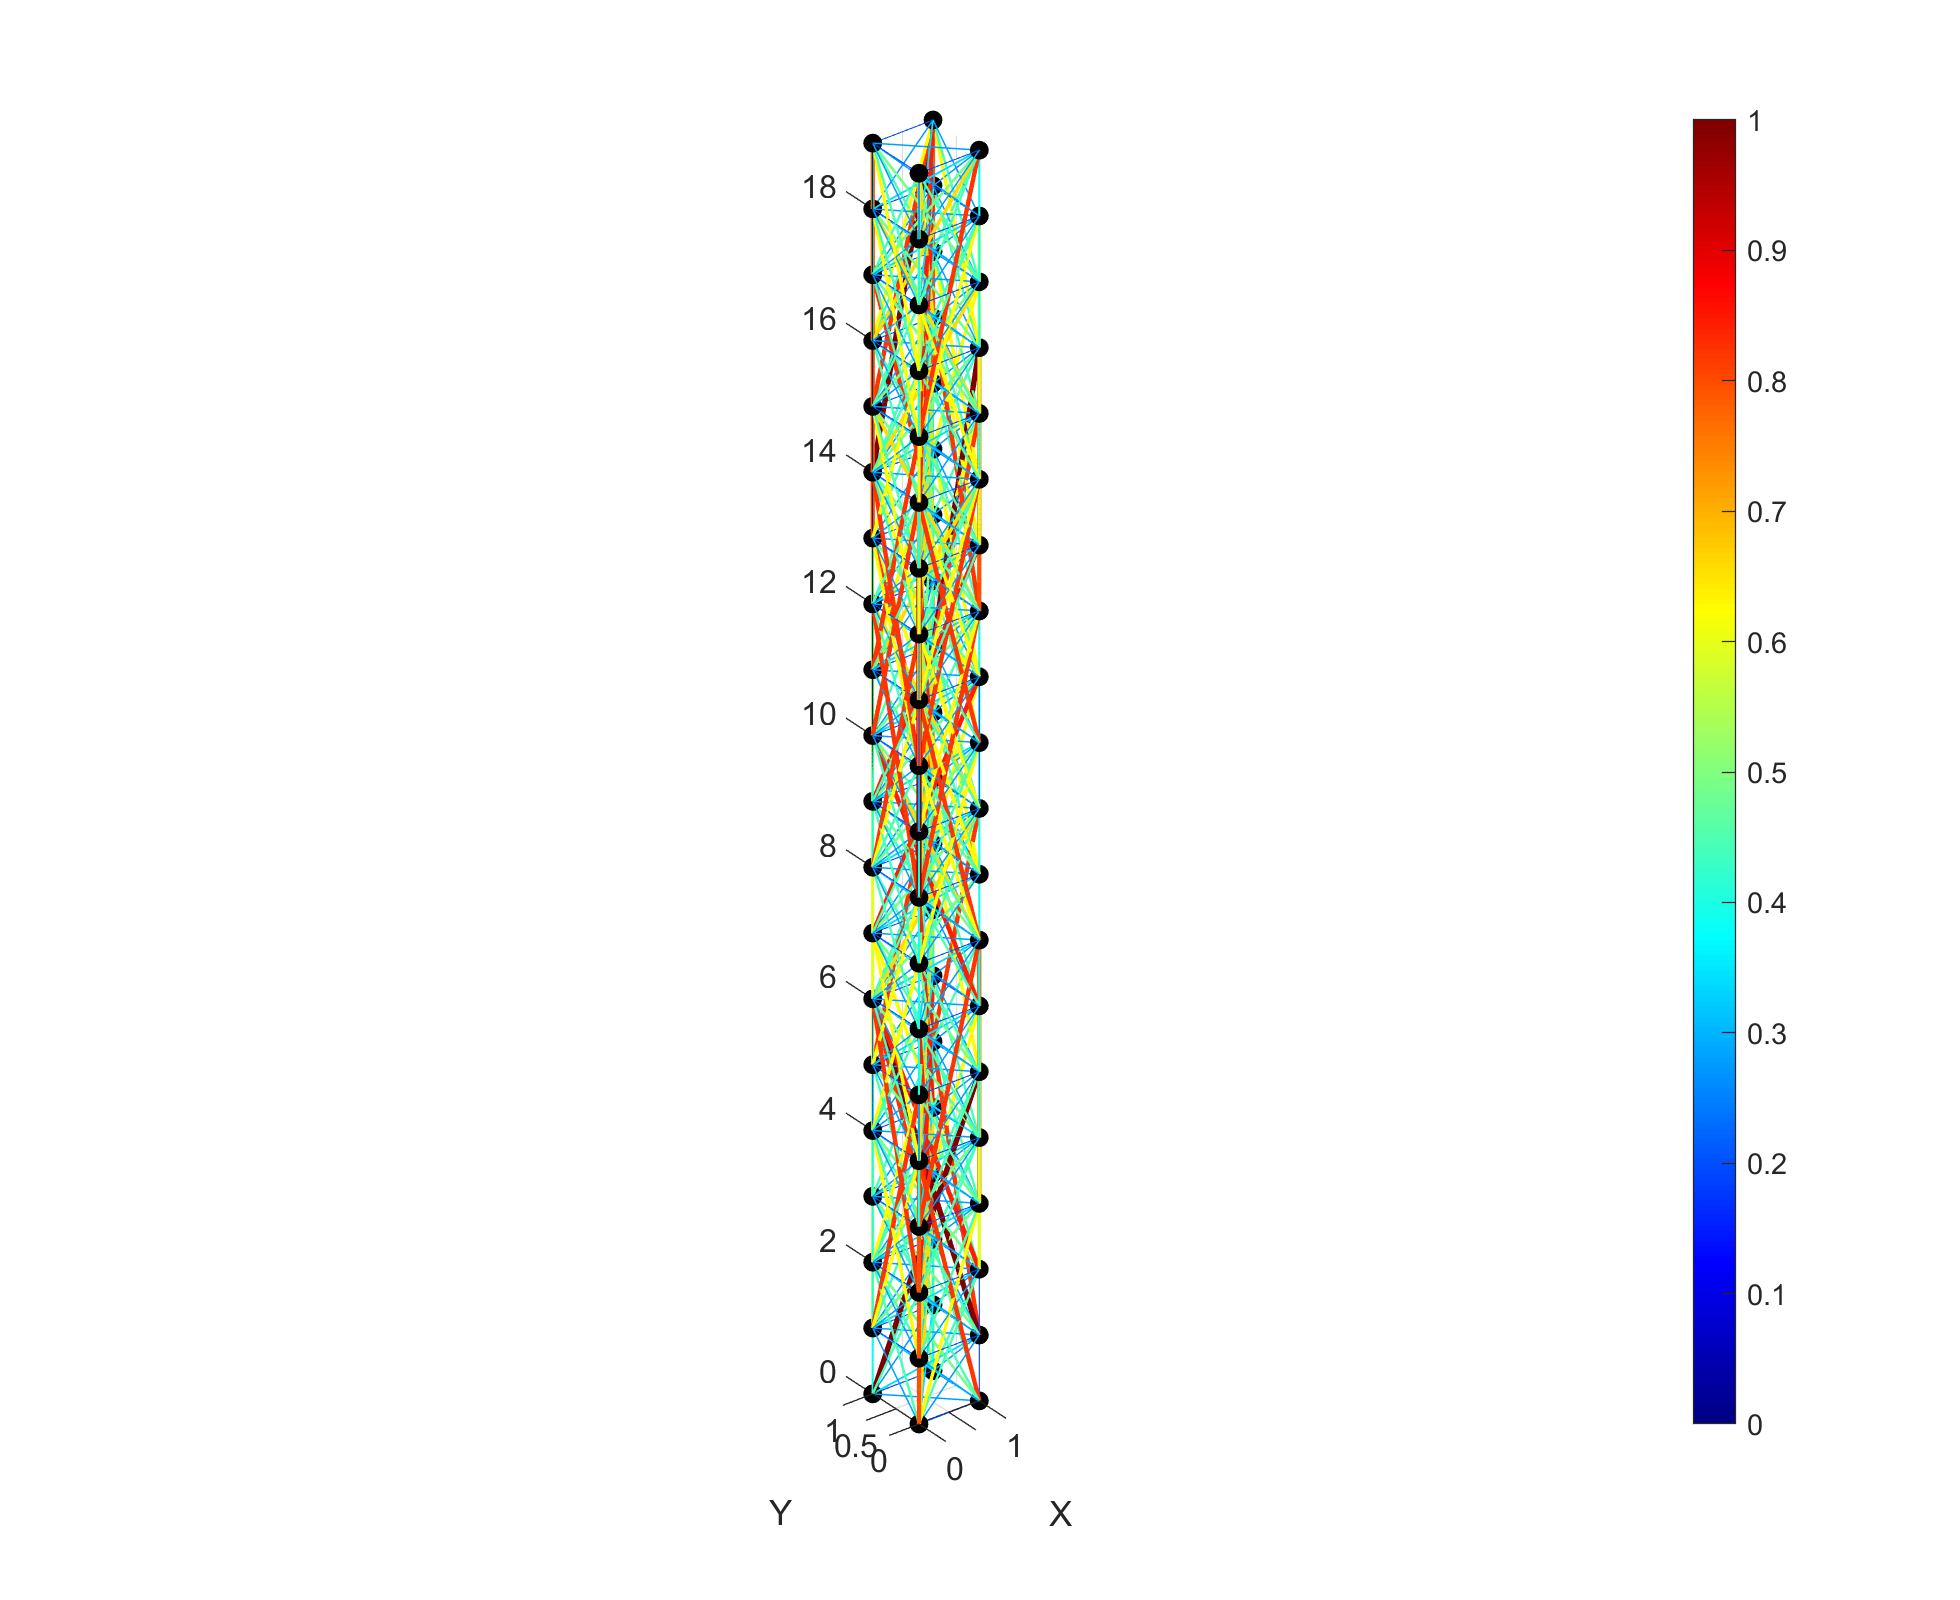
\includegraphics[height=2in]{fig/1D_Connection_Plot}
    \end{subfigure}
    \begin{subfigure}[b]{0.4\textwidth}
      \centering
      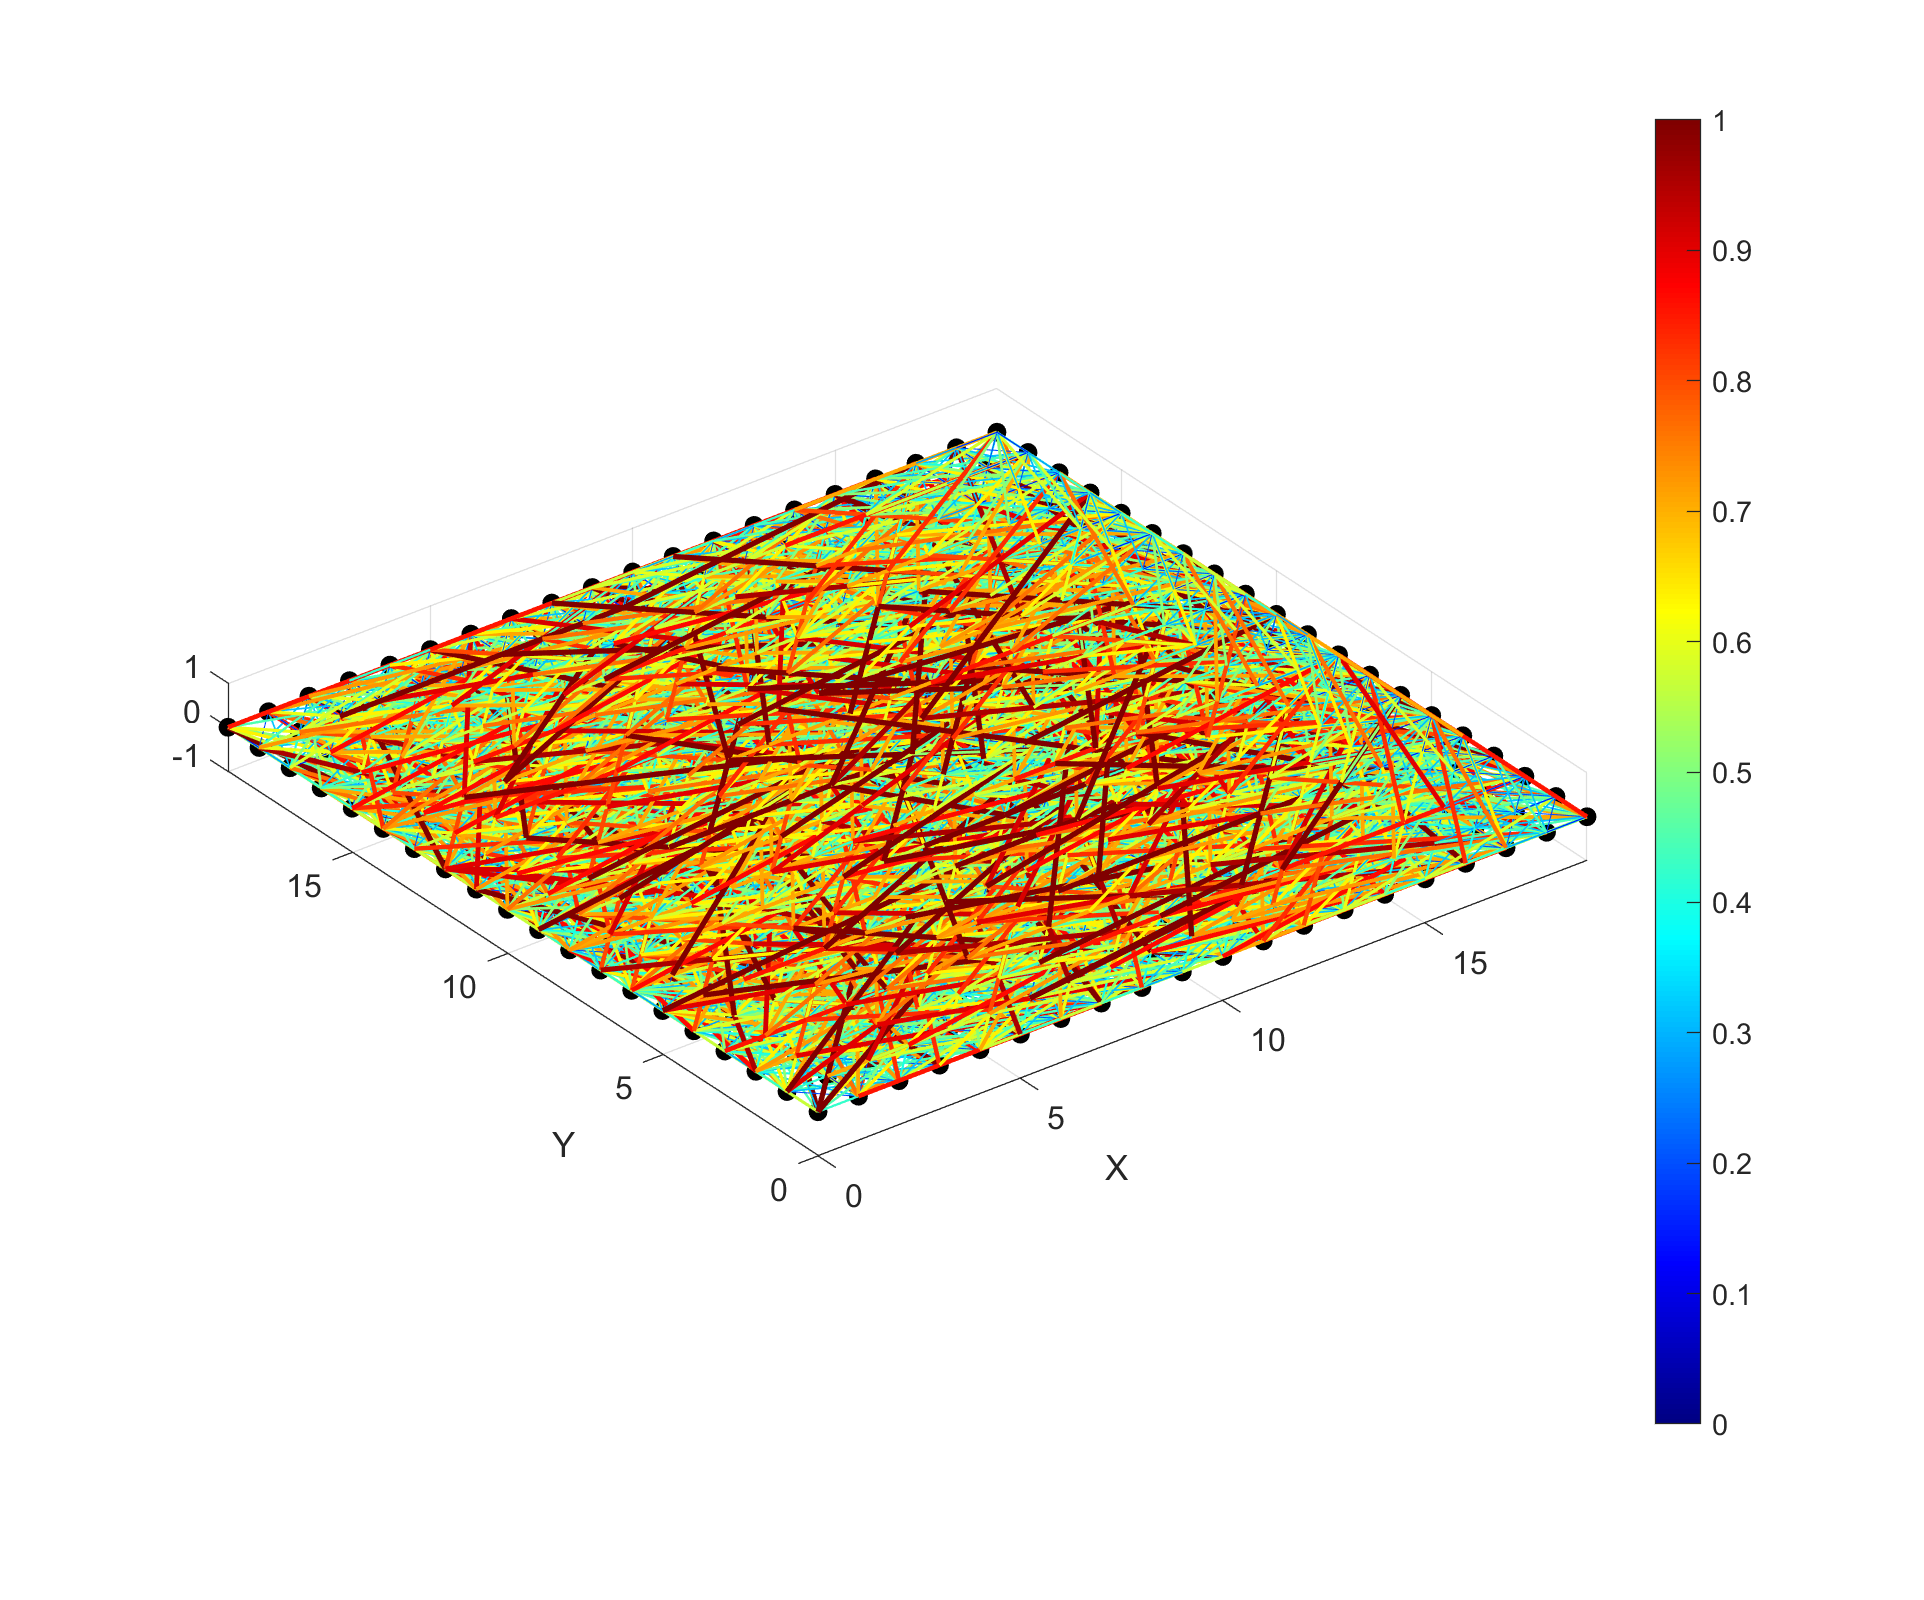
\includegraphics[height=2in]{fig/2D_Connection_Plot}
    \end{subfigure}
\end{figure}

In both types of circuit the neurons are connected with a strong local connectivity according to the distance-based connection probability:
\begin{align}\label{eq:connectivity}
 P_{a,b} &= C \times e^{-(D(a,b)/\lambda)^2}
\end{align}
Where $D(a,b)$ is the distance between neuron A and B and $\lambda$ and $C$ are parameters of the connection model.

We model the neurons using the Izhikevich model \cite{izhikevich2003} to allow us to explore the neural dynamics.
The Izhikevich model uses two coupled differential equations with two variables and four parameters:
\begin{align}
 v^\prime &= 0.04v^2+5v+140-u+I \label{eq:neuron_v} \\
 u^\prime &= a(bv-u)\\
 \text{if } &v>30: v\leftarrow c, u\leftarrow u+d
\end{align}
This is a simplified model of a two-dimensional dynamical system.
This model has been used to reproduce common neural firing patterns.
There is MATLAB code available \cite{izzy_code} that implements this neural model with fixed, single-time-step action potential propagation.
The model parameters for excitatory and inhibitory neurons are shown in Table \ref{tab:izzy_params}.
We define $\mathcal{U}\{a,b \}$ as a uniform random variable drawn on $[ a,b ] $.
\begin{table}[!ht]
 \caption{Izhekevich model parameters}
 \label{tab:izzy_params}
 \centering
 \begin{tabular}{l|c|r}
  \textbf{Parameter} & \textbf{Excitatory} & \textbf{Inhibitory} \\
  \hline
  a & 0.02 & 0.02+$\mathcal{U}$(0,0.08) \\
  b & 0.2 & 0.25-$\mathcal{U}(0,0.05)$\\
  c & -65+$\mathcal{U}(0,10)^2$ & -65 \\
  d & 8-$\mathcal{U}(0,6)$& 2 \\
 \end{tabular}
\end{table}
The distribution of model parameters represents the different types of neurons found in the cortex.
The excitatory neuron parameters create a mix of regular spiking, intrinsically bursting and chattering behavior.
The inhibitory neuron parameters create a mix of low-threshold spiking and fast spiking behavior \cite{izhikevich2003}.

In the Izhikevich model when a neuron fires the action potential propagates to the target neuron at the next time step.
The action potential from the firing neuron is added to the target neuron current $I$ (Eq \ref{eq:neuron_v}).
We enhanced the available MATLAB code for the Izhikevich model to incorporate a more realistic propagation model while still minimizing computational complexity.
Our model incorporates a propagation delay $\tau_{ij}=\kappa D(i,j)$ porportional to the inter-neuron distance $D(i,j)$ between neurons $i$ and $j$. 
The parameter $\kappa$ ranges from 0 (action potentials propagate to the target neuron in the next time step) to 4. 
We also model an exponentially decaying synapse respone $I(t)=e^{-(\frac{t}{\sigma_s})^2}$ with a time constant of $\sigma_s=4~ms$.

The connection strengths between neurons is based on the original Izhikevich work.
The strength for connections from presynaptic neuron $i$ to postsynaptic neuron $j$ depends on whether $i$ is inhibitory or excitatory.
\begin{align}
 S_{ij}^{excitatory} &= K \times \mathcal{U}\{0,\frac{1}{2} \} \\
 S_{ij}^{inhibitory} &= K \times \mathcal{U}\{-1,0 \} 
\end{align}
The parameter K is used to adjust the overall connection strength: $K=1$ corresponds to the original model in \cite{izzy_code}. 

The current in Equation \ref{eq:neuron_v} includes all incoming stimulus from other neurons.
With our models for action potential propagation and synapse response, the total current to neuron $i$ can be written:
\begin{align}
 I_i(t) &= \sum_{j\ne i} \sum_{t^\prime_j} S_{ij}  \Theta(t-t^\prime_j-\tau_{ij})e^{-(\frac{t-t^\prime_j-\tau_{ij}}{\sigma_s})^2}
\end{align}
Where the $t^\prime_j$ are all firing times of neuron $j$ and $\Theta$ is the Heaviside step function.

The current in Equation \ref{eq:neuron_v} also includes any stimulus applied as part of the experiment.
We perform experiments using both a uniform background stimulus and a step stimulus.
Our model for uniform background stimulus to a neuron $i$ depends on whether $i$ is inhibitory or excitatory, following Izhikevich's original model.
The uniform background stimulus is:
\begin{align}
 I_i^{excitatory} &= M \times \mathcal{U}\{0,1 \} \\
 I_i^{inhibitory} &= \frac{2}{5} M \times \mathcal{U}\{0,1 \}
\end{align}
The parameter $M$ is used to adjust the overal strength of the stimulus, $M=1$ corresponds to the original model in \cite{izzy_code}.

\section{Results}

We have observed preferential wave initiation sites in our experiments.
To understand the initiation mechanisms in our column model we first examine connectivity.
Figure \ref{fig:initiation_baseline} shows the firing of a typical column compared to the same column with all inter-neuron connections removed.
The unconnected column is stimulated with a different draw of the random background stimulus.
The unconnected column shows regions with higher firing activity that correspond to initiation sites in the connected column.
This indicates that the preferential firing sites are likely related to individual neuron dynamics and not inter-neuron connectivity.
\begin{figure}[!htb]
 \caption{Left: A typical column experiment showing preferential wave initiation near $Z=8$ and $Z=35$. Center: the same column with all inter-neuron connections removed. Right: Histogram of firing events by Z position in the disconnected column.}
 \label{fig:initiation_baseline}
 \centering
   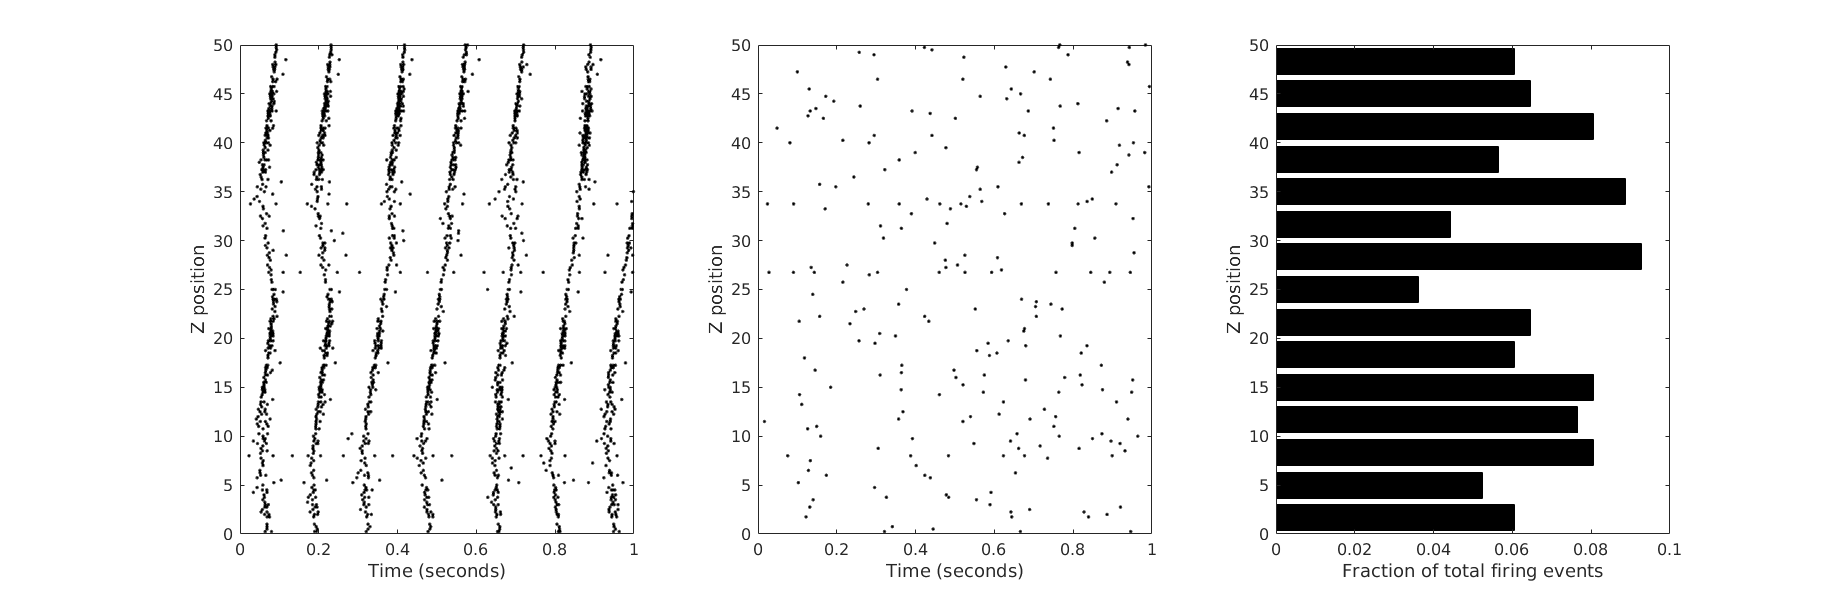
\includegraphics[width=\textwidth]{fig/InitiationBaseline}
\end{figure}

The $b$ parameter in the Izhikevich model sets the firing threshold of the individual neurons.
Per Table \ref{tab:izzy_params} excitatory neurons all have a $b$ parameter of $0.2$, while inhibitory neurons have $b$ parameters in the range $0.2-0.25$.
Neurons with higher $b$ parameter are easier to excite and therefore more likely to fire.
It may seem counter-intuitive that firing activity from an inhibitory neuron would generate traveling waves.
In fact, postinhibitory rebound spiking is commonly observed in coritcal neurons \cite{ascoli2010} and is observed in the Izhikevich model of neuron dynamics \cite{izhikevich}.

In general only some of the neurons in the column will fire when a wave passes.
We observed that a single traveling wave can have regions of higher or lower total firing activity, which we term firing density.
An example measurement of the firing activity in a single traveling wave is shown in Figure \ref{fig:wave_density}.
\begin{figure}[!htb]
 \caption{Density of firing events in a traveling wave initiated from a step stimulus. The traveling wave is shown on the left, a histogram of firing events by position is shown on the right.}
 \label{fig:wave_density}
 \centering
   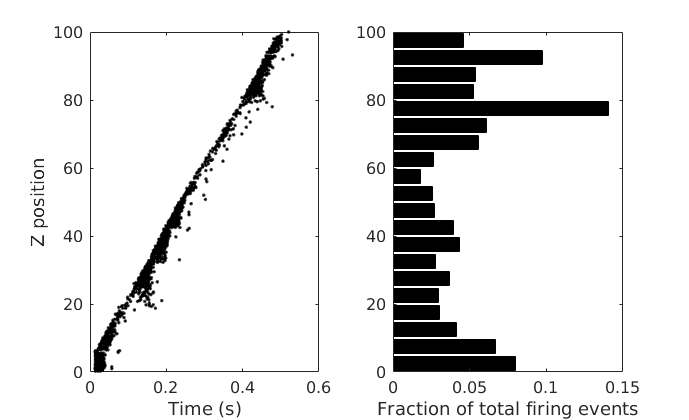
\includegraphics[width=0.75\textwidth]{fig/ImpulseWaveDensity}
\end{figure}

While examining the preferential wave initiation sites emerging from random stimulus we discovered a negative correlation to the firing density observed in a single wave generated by a step stimulus.
The wave initiation sites and wave density of the same column are shown in figure \ref{fig:initiation_density}.
This visually illustrates that the preferential firing sites tend towards lower firing density in the single wave experiments.
\begin{figure}[!htb]
 \caption{Wave initiation (left) and wave density (right) for the same column.}
 \label{fig:initiation_density}
 \centering
   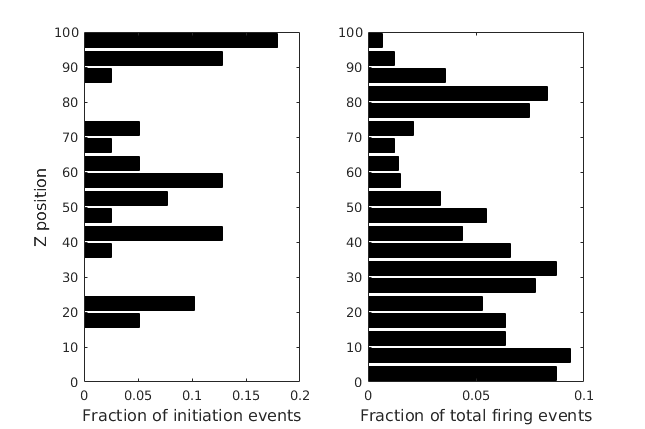
\includegraphics[width=0.75\textwidth]{fig/InitiationCorrelationHistogram}
\end{figure}

To test this hypothesis we create 100 columns, applied both uniform background stimulus and step stimulus to each column, and measured the correlation between wave inititation and firing density at the positions of the column (Figure \ref{fig:initiation_density_corr}).
Although there is substantial variation between columns we measure a consistently negative correlation coefficient (mean -0.18, std 0.20).
We expect that the lower firing density is caused by the low-threshold inihibitory neurons at those sites that are responsible for generating traveilng waves under uniform background stimulus.
\begin{figure}[!htb]
 \caption{Correlation between wave initiation and wave density.}
 \label{fig:initiation_density_corr}
 \centering
   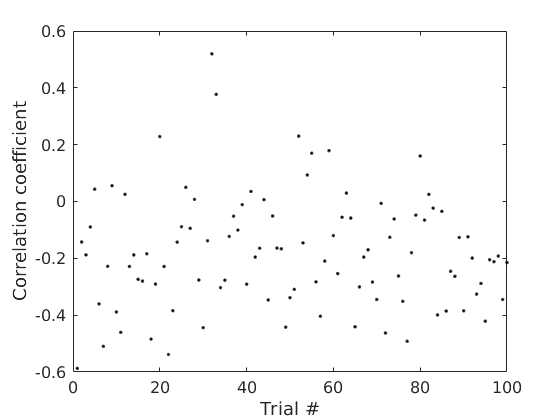
\includegraphics[width=0.75\textwidth]{fig/InitiationCorrelation}
\end{figure}

To demonstrate that the low-threshold spiking inhibitory neurons are responsible for generating traveling waves under background stimulus and suppressing firing activity inside a single traveling wave we performed a final experiment.
We created a column with entirely excitatory neurons except for a single LTS inhibitory neuron with $b=25$ at $Z=40$.
This column was stimulated with both a uniform background stimulus and a step stimulus. 
Figure \ref{fig:lts_inhibit} clearly shows that the single LTS neuron generates traveling waves emanating from $Z=40$. 
A traveling wave does emerge near $Z=23$ at the beginning of the experiment, but the regular traveling waves triggered by the LTS neuron dominate the firing activity.
The wave density at $Z=40$ is the minimum density within the traveling wave, confirming that the LTS neuron also suppresses firing activity in a passing traveling wave.
\begin{figure}[!htb]
 \caption{Experiment with a single LTS inhibitory neuron at $Z=40$. Left: Traveling waves are initiated byt the LTS inhibitory neuron. Center: a single traveling wave generated by a step stimulus. Right: The traveling wave density is minimum at $Z=40$.}
 \label{fig:lts_inhibit}
 \centering
   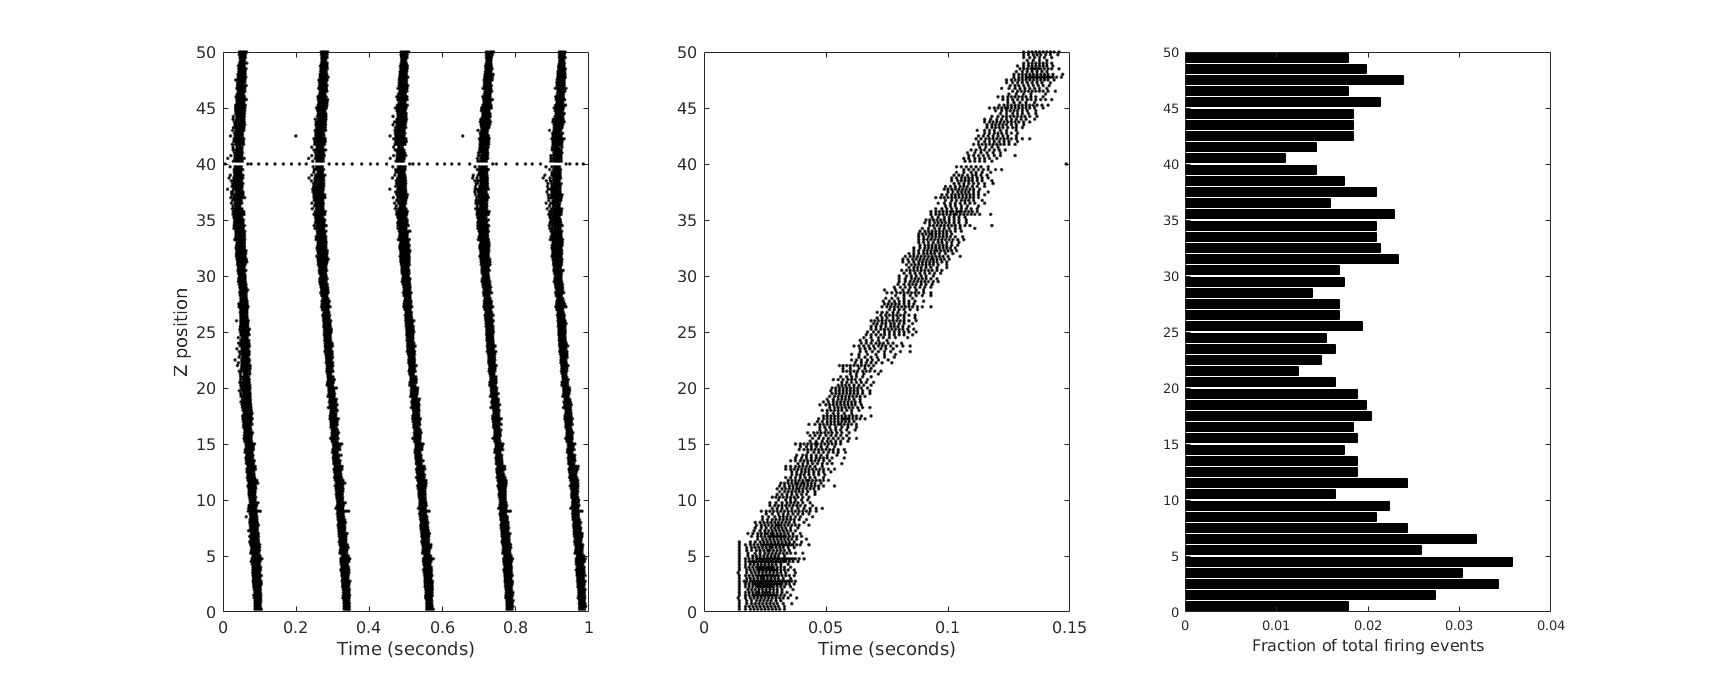
\includegraphics[width=\textwidth]{fig/SingleLTSInhibit}
\end{figure}


\section{Discussion}
Our model shows preferential sites for wave initiation due to the presence of inhibitory neurons with low spiking thresholds.
Low-threshold inhibitory neurons in the Izhikevich model represent the low-threshold spiking inhibitory neurons that are found in the cortex \cite{izhikevich2003}\cite{gibson2009}.
These low-threshold neurons could act as ''pacemakers'' for traveling waves in the cortex, providing spatial and temporal synchronization.

\clearpage
\printbibliography

\end{document}
